%\documentclass[10pt]{beamer}
\documentclass[handout,10pt]{beamer}


\usetheme[progressbar=frametitle]{metropolis}

\usepackage{booktabs}
\usepackage[scale=2]{ccicons}


\usepackage{amsmath}
\usepackage{pgfplots}
\usepgfplotslibrary{dateplot}

\usepackage{xspace}
\newcommand{\themename}{\textbf{\textsc{metropolis}}\xspace}

%\usepackage{placeins} %%%
\usepackage{subfig}
\usepackage{physics}
\usepackage{amssymb}


\usepackage{tikz}
\usepackage{circuitikz}
\usepackage{siunitx}


\usepackage{latexsym}
\usepackage{mathtools}
\usepackage{slashed} % for the Feynman slash notation

\usepackage{listings}

\usepackage{balance}


% edited by Mauro 28-12-16
%
%% <local definitions>
\newcommand{\R}{\mathbb{R}}	
\newcommand{\C}{\mathbb{C}}
\newcommand{\HQ}{\mathbb{H}}
\newcommand{\N}{\mathbb{N}}
\newcommand{\be}{\begin{equation}}
\newcommand{\ee}{\end{equation}}	
\newcommand{\bea}{\begin{eqnarray}}
\newcommand{\eea}{\end{eqnarray}}	
\newcommand{\Pin}{\mathrm{Pin}}	
\newcommand{\Spin}{\mathrm{Spin}}
\renewcommand{\O}{\mathrm{O}}
\newcommand{\SO}{\mathrm{SO}}
\renewcommand{\eqref}[1]{(\ref{#1})}
\newcommand{\cl}[1]{\ensuremath{Cl(#1)}} % #1 stands for the values p,q. $\cl{p,q}$ produces 'Cl(p,q)'.
\newcommand{\gvec}[1]{\ensuremath{\mbox{\textbf{\textit{#1}}}}}
\newcommand{\vect}[1]{\ensuremath{\mbox{\textbf{\textit{#1}}}}}
%% </local definitions>

\newcommand{\Ba}[0]{\mathbf{a}}
\newcommand{\Bb}[0]{\mathbf{b}}
\newcommand{\Bc}[0]{\mathbf{c}}
\newcommand{\Bd}[0]{\mathbf{d}}
\newcommand{\Be}[0]{\mathbf{e}}
\newcommand{\Bf}[0]{\mathbf{f}}
\newcommand{\Bg}[0]{\mathbf{g}}
\newcommand{\Bh}[0]{\mathbf{h}}
\newcommand{\Bi}[0]{\mathbf{i}}
\newcommand{\Bj}[0]{\mathbf{j}}
\newcommand{\Bk}[0]{\mathbf{k}}
\newcommand{\Bl}[0]{\mathbf{l}}
\newcommand{\Bm}[0]{\mathbf{m}}
\newcommand{\Bn}[0]{\mathbf{n}}
\newcommand{\Bo}[0]{\mathbf{o}}
\newcommand{\Bp}[0]{\mathbf{p}}
\newcommand{\Bq}[0]{\mathbf{q}}
\newcommand{\Br}[0]{\mathbf{r}}
\newcommand{\Bs}[0]{\mathbf{s}}
\newcommand{\Bt}[0]{\mathbf{t}}
\newcommand{\Bu}[0]{\mathbf{u}}
\newcommand{\Bv}[0]{\mathbf{v}}
\newcommand{\Bw}[0]{\mathbf{w}}
\newcommand{\Bx}[0]{\mathbf{x}}
\newcommand{\By}[0]{\mathbf{y}}
\newcommand{\Bz}[0]{\mathbf{z}}
\newcommand{\BA}[0]{\mathbf{A}}
\newcommand{\BB}[0]{\mathbf{B}}
\newcommand{\BC}[0]{\mathbf{C}}
\newcommand{\BD}[0]{\mathbf{D}}
\newcommand{\BE}[0]{\mathbf{E}}
\newcommand{\BF}[0]{\mathbf{F}}
\newcommand{\BG}[0]{\mathbf{G}}
\newcommand{\BH}[0]{\mathbf{H}}
\newcommand{\BI}[0]{\mathbf{I}}
\newcommand{\BJ}[0]{\mathbf{J}}
\newcommand{\BK}[0]{\mathbf{K}}
\newcommand{\BL}[0]{\mathbf{L}}
\newcommand{\BM}[0]{\mathbf{M}}
\newcommand{\BN}[0]{\mathbf{N}}
\newcommand{\BO}[0]{\mathbf{O}}
\newcommand{\BP}[0]{\mathbf{P}}
\newcommand{\BQ}[0]{\mathbf{Q}}
\newcommand{\BR}[0]{\mathbf{R}}
\newcommand{\BS}[0]{\mathbf{S}}
\newcommand{\BT}[0]{\mathbf{T}}
\newcommand{\BU}[0]{\mathbf{U}}
\newcommand{\BV}[0]{\mathbf{V}}
\newcommand{\BW}[0]{\mathbf{W}}
\newcommand{\BX}[0]{\mathbf{X}}
\newcommand{\BY}[0]{\mathbf{Y}}
\newcommand{\BZ}[0]{\mathbf{Z}}

\newcommand{\ta}[0]{\tilde{a}}
\newcommand{\tb}[0]{\tilde{b}}
\newcommand{\tc}[0]{\tilde{c}}
\newcommand{\td}[0]{\tilde{d}}

\newcommand{\hA}[0]{\hat{A}}
\newcommand{\hB}[0]{\hat{B}}
\newcommand{\hH}[0]{\hat{H}}

\newcommand{\tA}[0]{\tilde{A}}
\newcommand{\tB}[0]{\tilde{B}}
\newcommand{\tF}[0]{\tilde{F}}
\newcommand{\tE}[0]{\tilde{E}}
\newcommand{\tH}[0]{\tilde{H}}

% spinors definition
\newcommand{\barJ}[0]{\bar{J}}
\newcommand{\barF}[0]{\bar{F}}
\newcommand{\barP}[0]{\bar{P}}
\newcommand{\barW}[0]{\bar{W}}



\newcommand{\tnabla}[0]{\tilde{\nabla}}
\newcommand{\tphi}[0]{\tilde{\phi}}
\newcommand{\tpsi}[0]{\tilde{\psi}}

%
\newcommand{\wavep}[0]{\partial^+}
\newcommand{\wavem}[0]{\partial^-}

\newcommand{\wavepp}[0]{\tilde{\partial}^+}
\newcommand{\wavemp}[0]{\tilde{\partial}^-}

\newcommand{\wavepd}[0]{\bar{\partial}^+}
\newcommand{\wavemd}[0]{\bar{\partial}^-}

\newcommand{\pbd}[0]{\bar{\partial}_d}

% frequency

\newcommand{\helmp}[0]{{\underline{\partial}}^+}
\newcommand{\helmm}[0]{{\underline{\partial}}^-}

\newcommand{\helmpp}[0]{{\underline{\tilde{\partial}}}^+}
\newcommand{\helmmp}[0]{{\underline{\tilde{\partial}}}^-}

\newcommand{\helmpd}[0]{{\underline{\bar{\partial}}}^+}
\newcommand{\helmmd}[0]{{\underline{\bar{\partial}}}^-}

\newcommand{\pbfd}[0]{{\underline{\bar{\partial}}}_d}




\def \figname {Figure}
\def \emode {E }
\def \hmode {H }
\def \temode {TE }
\def \tmmode {TM }
\def \temoden {TE${}_n$ }
\def \tmmoden {TM${}_n$ }
\def \temodemn {TE${}_{mn}$ }
\def \tmmodemn {TM${}_{mn}$ }



\newcommand{\iGA}{{i}}
\newcommand{\conjg}[1] {\ensuremath{#1}^*}

\setbeamertemplate{bibliography item}{[\theenumiv]}


\title{Dirac matrices}

\date{}

%\subtitle{Maximizing efficiency and power at a fixed frequency}
%\date{\today}
%\author{Alessandra Costanzo, Franco Mastri, Mauro Mongiardo*, Giuseppina Monti}
%\institute{*Department of Engineering,
%University of Perugia, Italy}

\author{ Mauro Mongiardo$^1$}

\institute{
 $^1$ Department of Engineering, University of Perugia, Perugia, Italy.
}

%
\titlegraphic{\hfill\includegraphics[height=1.5cm]{logo}}


\begin{document}

\maketitle

\begin{frame}{Table of contents}
  \setbeamertemplate{section in toc}[sections numbered]
  \tableofcontents[hideallsubsections]
\end{frame}

%=========================================================================
\section{Introduction}
%=========================================================================

%=========================================================================
\begin{frame}[fragile]{}

Traditional vector analysis relies on the approach proposed by Gibbs at the beginning of 1900 \cite{gibbs} and generally adopted in electromagnetic field engineering.

Later, several different approaches have been presented and elucidated.

As an example differential forms \cite{russer} and Geometric or Clifford Algebra, in the following briefly referred to as GA \cite{hestenes}\cite{seagar}. 

\alert{Generally GA has been employed in electromagnetic (EM) by considering the point of view of physicists and not of engineers \cite{arthur}\cite{abbott}.}

As an example, in EM  engineering  wide use is made of time--harmonic analysis \cite{harrington}, while no publication deals with application of GA to the time--harmonic regime.

\end{frame}


\begin{frame}[allowframebreaks]{References}


\begin{thebibliography}{99}
%----------------------------------------------------------------------------------------------------------------------------------------------
%
%\bibliographystyle{IEEEtran}
%\bibliography{WLPT,wireless_power_transmission,topology}
\bibitem{gibbs}J. W. Gibbs, \emph{Elements of Vector Analysis}, Tuttle, Morehouse \& Taylor, 1884;
\bibitem{russer}P. Russer, \emph{Exterior Differential Forms in Teaching Electromagnetics} in \emph{Electromagnetics in a Complex World - Challenges and Perspectives}, Springer, 2004;
\bibitem{hestenes}D. Hestenes, G. Sobczyk, \emph{Clifford Algebra to Geometric Calculus: A Unified Language for  Mathematics and Physics}, Dordrecht: Kluwer Academic Publishers, 1987;

\bibitem{seagar}A. Seagar, \emph{Application of Geometric Algebra to Electromagnetic scattering: The Clifford--Cauchy--Dirac Technique}, Springer Publishing Companys, 2015;


\bibitem{arthur}J. W. Arthur, \emph{Understanding Geometric Algebra}, New York: Wiley-IEEE, 2011;
\bibitem{abbott}J. M. Chappell et al., "Geometric Algebra for Electrical and Electronic Engineers," in Proceedings of the IEEE, vol. 102, no. 9, pp. 1340-1363, Sept. 2014. doi: 10.1109/JPROC.2014.2339299;

\bibitem{abbott2}J. M. Chappell, A. Iqbal, J. G. Hartnett and D. Abbott, "The Vector Algebra War: A Historical Perspective," in IEEE Access, vol. 4, no. , pp. 1997-2004, 2016.
doi: 10.1109/ACCESS.2016.2538262

\bibitem{harrington}R.F. Harrington, \emph{Time-Harmonic Electromagnetic Fields}, IEEE-Press, 2001;

%,Cambridge_journal
%----------------------------------------------------------------------------------------------------------------------------------------------
%
\end{thebibliography}
\end{frame}

%%%%%%%%%%%%%%%%%%%%%%%%%%%%%%%%%%%%%%%%%%




%%%%%%%%%%%%%%%%%%%%%%%%%%%%%%%%%%%%%%%%%%%

%=========================================================================
\begin{frame}[shrink=20]{As appeared in \cite{abbott2}}

\begin{center}
\begin{figure}

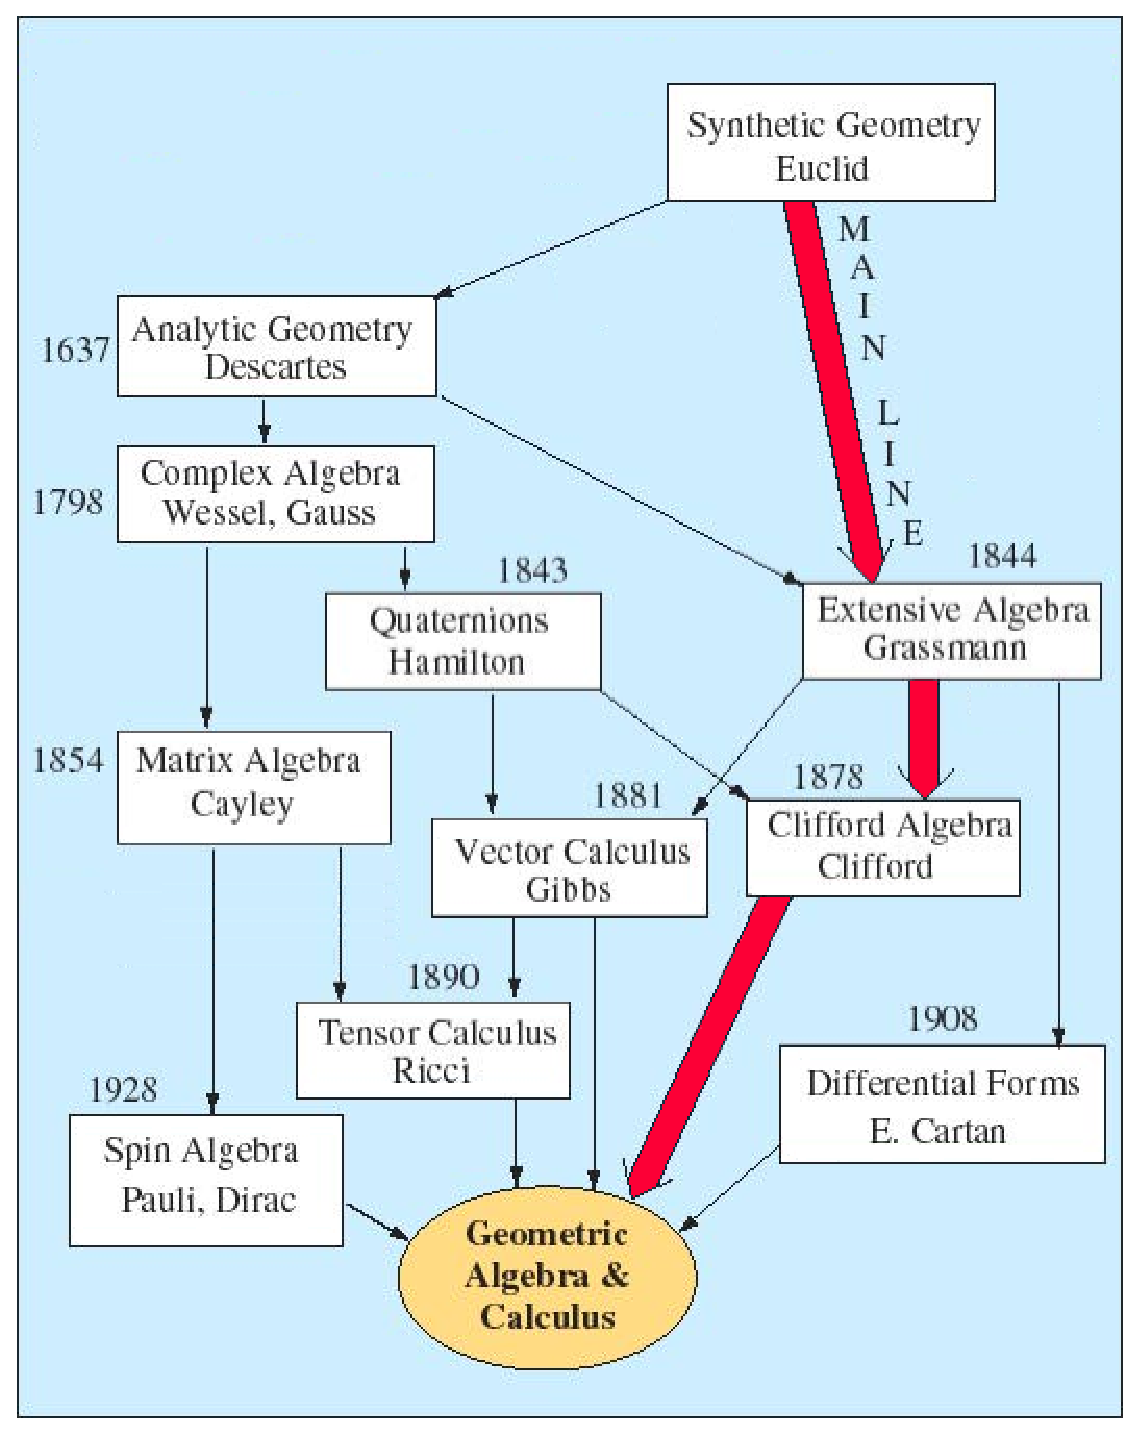
\includegraphics[scale=0.47]{DescentVectors}

\caption{\label{DescentOfVectors} The descent of the various vector systems. The main path of development beginning from Euclid geometry down through Grassman and then to Clifford. Other parallel developments using complex numbers, quaternions, Gibbs' vectors, tensors, matrices and spinor algebra subsumed into the general formalism of Clifford geometric algebra with the inclusion of calculus.}
\end{figure}
\end{center}

\end{frame}


%=========================================================================
\begin{frame}[fragile]{}

Most of the engineering EM analysis are performed in a three--dimensional space (3D). 
In the 3D space a very interesting fact takes place: \alert{GA is equivalent to Pauli algebra}.

Pauli matrices have been introduced by Wolfgang Pauli 
%(https://en.wikipedia.org/wiki/Wolfgang_Pauli) 
for the spin theory.

Very remarkably, \alert{by using Pauli matrices a vector can be represented as a 2x2 matrix}. 
Thus it is possible to multiply vectors by multiplying the relative matrices. 

\alert{It is also possible to make the inverse of a vector!}
\end{frame}

%=========================================================================
\begin{frame}[fragile]{GA in 3D and Pauli matrices}

In the 3D space, according to GA, we need to represent:
\alert{
\begin{itemize}
\item a scalar;
\item 3 vectors;
\item 3 bivectors;
\item psuedo--scalar
\end{itemize}
}
 i.e. 8 numbers. 

It is possible to introduce a \alert{multivector} which is the sum of a scalar, a vector, a bivector and a pseudo--scalar. 

Such multivector can be represented by a 2x2 matrix and can be constructed in terms of Pauli matrices. 

\end{frame}

%=========================================================================
\begin{frame}[shrink=25]{}

\begin{figure}[htb]
\begin{center}
\includegraphics[width=3.5in]{GeometrySpace}
\end{center}
\caption{Identify the basis vectors as $e_1 = \sigma_1$, $e_2 = \sigma_2$, $e_3 = \sigma_3$.These are elements of Clifford's model for three--dimensional space. This consists of three unit vectors $ e_1, e_2 $ and $ e_3 $, three unit areas $ e_2 e_3, e_3 e_1 $ and $ e_1 e_2 $ and a unit volume $ \iGA = e_1 e_2 e_3 $. The pure scalars then defining points to form a complete algebraic description of three-dimensional physical space. \label{ThreeSpace}}
\end{figure}
\end{frame}
%=========================================================================
 \section{Pauli matrices and their properties}
 
 
%=========================================================================
\begin{frame}[shrink=10]{Wolfgang Pauli}
\begin{figure}[htb]

\begin{center}
\includegraphics[width=1.0in]{220px-Pauli}
\end{center}

\caption{Wolfgang Pauli}

Wolfgang Ernst Pauli (25 April 1900 -- 15 December 1958) was an Austrian-born Swiss and American theoretical physicist and one of the pioneers of quantum physics. 

In 1945, after having been nominated by Albert Einstein, Pauli received the Nobel Prize in Physics for his "decisive contribution through his discovery of a new law of Nature, the exclusion principle or Pauli principle". 

%The discovery involved spin theory, which is the basis of a theory of the structure of matter.
\end{figure}

\end{frame}


%=========================================================================
\begin{frame}[fragile]{Pauli matrices}



We first introduce the Pauli matrices and then discuss some of their properties and show how to operate with this new tool.

Note that engineers are quite well trained to operate with matrices and we will see that many standard vectors operations can be simplified and new important elements will be found.

 The Pauli matrices are a set of three 2x2 complex matrices which are \emph{Hermitian} and \emph{unitary}. 
 
  The Pauli matrices have the following form
%
\begin{eqnarray}
\sigma_1 &= & \begin{pmatrix}0 & 1\cr 1 & 0\end{pmatrix} \nonumber \\
%
\sigma_2 &= & \begin{pmatrix}0 & -i\cr i & 0\end{pmatrix} \nonumber \\
%
\sigma_3 &= &\begin{pmatrix}1 & 0\cr 0 & -1\end{pmatrix}  \, .
%
\end{eqnarray}
%

\end{frame}

%=========================================================================
\begin{frame}[fragile]{Properties of the Pauli matrices}

It is immediately noted that the trace of these matrices is always zero. 

The determinant of the Pauli matrices is always -1.

The following products hold: 
%
\begin {equation}
\sigma_1^2 = \sigma_2^2 = \sigma_3^2 =  \begin{pmatrix}1 & 0\cr 0 & 1\end{pmatrix} = I = \sigma_0\,.
 \end{equation}
 %
By multiplying e.g. $\sigma_1$ with $\sigma_2$ the result is $i \sigma_3$ and similarly for the other cases:
%
\begin {eqnarray}
\sigma_1 \sigma_2 &=& i \sigma_3  = - \sigma_2 \sigma_1 \nonumber \\
\sigma_2 \sigma_3 &=& i \sigma_1 =  - \sigma_3  \sigma_2\nonumber \\
\sigma_3 \sigma_1 &=&  i \sigma_2 =  - \sigma_1  \sigma_3 \,.
\label{sigmacomb}
 \end{eqnarray}
 %

\end{frame}

%=========================================================================
\begin{frame}[fragile]{}
The above relations are very important. In fact, they show that, in the three-dimensional case, we can always replace the quantities $\sigma_i\sigma_j$ with the orthogonal vector $i \sigma_k$.
% (with the appropriate combination given in (\ref{sigmacomb})).
 
 From the above properties it is seen that
 \be\label{i123}
 (\sigma_1 \sigma_2 \sigma_3)^2 =  \sigma_1 \sigma_2 \sigma_3 \sigma_1 \sigma_2 \sigma_3 = -1 \
 \ee
i.e. $ \sigma_1 \sigma_2 \sigma_3 = i$.
 
The three Pauli matrices, with the addition of the identity matrix $\sigma_0$, form a basis in the space of the 2x2  Hermitian matrices and a matrix $A$ can be represented as:
%
\begin {equation}
A = a_0\sigma_0 + a_1 \sigma_1 + a_2 \sigma_2 + a_3 \sigma_3\,.
 \end{equation}
 %
It is worthwhile to note that when the coefficients ($a_0,a_1,a_2,a_3$) are complex, also non Hermitian matrices can be described by the basis of ($\sigma_0,\sigma_1,\sigma_2, \sigma_3$).

\end{frame}

%=========================================================================
\begin{frame}[fragile]{The Pauli vector}


Let us introduce the Pauli vector which is a vector made by the three matrices ($\sigma_1,\sigma_2, \sigma_3$).
%
\begin {equation}
{\bf \sigma} = \left(  \sigma_1 \, {\bf x}_0,  \sigma_2 \, {\bf y}_0 ,  \sigma_3\, {\bf z}_0  \right)\,.
 \end{equation}
 %
We can consider the vector $\Ba = \left(a_x\, {\bf x}_0 +  a_y \, {\bf y}_0 + a_z \, {\bf z}_0 \right)$  in the three-dimensional space and make the following product:
%%
%\begin {equation}
%\tilde{a} = {\bf \sigma} \cdot {\bf a} = 
%\sigma_1 a_x + \sigma_2 a_y +\sigma_3 a_z
%=\begin{pmatrix}a_z & a_x - i a_y \cr a_x + i a_y & -a_z\end{pmatrix}\,
%\label{Epauli}
% \end{equation}
% %
 %%%%%%%%%%%%%%%%%%%%%%%%%%%%%%%%%%%%%%%%%

\bea
\tilde{a} &=& {\bf \sigma} \cdot {\bf a} = 
\sigma_1 a_x + \sigma_2 a_y +\sigma_3 a_z \\
& = &  \begin{pmatrix}0 & 1\cr 1 & 0\end{pmatrix} a_x +
\begin{pmatrix}0 & -i\cr i & 0\end{pmatrix} a_y +
\begin{pmatrix}1 & 0\cr 0 & -1\end{pmatrix} a_z  \\
& = &
\begin{pmatrix}a_z & a_x - i a_y \cr a_x + i a_y & -a_z\end{pmatrix}\,
\label{Epauli}
\eea
 
 
% \be
%\tnabla   =   \sigma \cdot \nabla = \sigma_1 \partial_x + \sigma_2 \partial_y +\sigma_3 \partial_z  \nonumber
%\ee

The matrix $\tilde{a}$ is an equivalent description of the vector ${\bf a}$ in terms of a 2x2 matrix. Two different symbols have been used to denote the 2x2 matrix representation $\tilde{a}$  and the standard vector representation ${\bf a}$. 
%They refer to exactly the same quantity and it is always possible to pass from one to the other. 

\end{frame}

%=========================================================================
\begin{frame}[shrink=20]
Let us try the product between two matrices $\ta, \tb$ and evaluate their product $\tc = \ta \tb$,
\bea
\tiny
\ta & = & \begin{pmatrix}a_3 & a_1-i\,a_2\cr i\,a_2+a_1 & -a_3\end{pmatrix} \nonumber \\
\tb & = &\begin{pmatrix}b_3 & b_1-i\,b_2\cr i\,b_2+b_1 & -b_3\end{pmatrix} \nonumber \\
\tc & = &\begin{pmatrix}a_3\,b_3+\left( a_2+i\,a_1\right) \,b_2+\left( a_1-i\,a_2\right) \,b_1 & \left( i\,a_2-a_1\right) \,b_3-i\,a_3\,b_2+a_3\,b_1\cr \left( i\,a_2+a_1\right) \,b_3-i\,a_3\,b_2-a_3\,b_1 & a_3\,b_3+\left( a_2-i\,a_1\right) \,b_2+\left( i\,a_2+a_1\right) \,b_1\end{pmatrix} \nonumber
\normalsize
\eea
%

\begin{itemize}
\item \alert{\emph{the trace of $\tc=\ta \tb$ divided by 2 gives us the dot product}}.
\end{itemize}
\be \label{dotpauli}
\Ba \cdot \Bb = 
(\tc_{11} + \tc_{22})/2 = a_1\,b_1+a_2\,b_2+a_3\,b_3
\ee

It is straightforward to recognize that the component along $x,y, z$ can be easily retrieved by the following operations
%
\bea
c_x & = & \frac{{c}_{21}+{c}_{12}}{2} \nonumber \\
c_y & = &  -\frac{i\,\left( {c}_{21}-{c}_{12}\right) }{2}\nonumber \\
c_z & = &  \frac{{c}_{11}-{c}_{22}}{2}
\eea
%

\end{frame}


%=========================================================================
\begin{frame}[shrink=20]

By writing them explicitly we find:
%
\bea
c_x & = & i\,\left( a_2\,b_3-a_3\,b_2\right)  \nonumber \\
c_y & = &  -i\,\left( a_1\,b_3-a_3\,b_1\right)  \nonumber \\
c_z & = &  i\,\left( a_1\,b_2-a_2\,b_1\right) 
\eea
%
It is now easy to recognize that, apart for the $i$ factor, this  is equal to the well known cross product.
This new part is called \alert{ \emph{external product} and is denoted by $\Ba \wedge \Bb$}. We have just obtained the important identity:
%
\be \label{epcross}
\Ba \wedge \Bb = i \, \Ba \times \Bb \, .
\ee
%
Naturally, to represent the wedge product in terms of the Pauli matrices it is sufficient to subtract the dot product from $\ta \tb$, thus obtaining
%
\be \label{epcrossexplicit}
\Ba \wedge \Bb = \begin{pmatrix}i\,\left( a_1\,b_2-a_2\,b_1\right)  & i\,a_2\,b_3-a_1\,b_3-i\,a_3\,b_2+a_3\,b_1\cr i\,a_2\,b_3+a_1\,b_3-i\,a_3\,b_2-a_3\,b_1 & -i\,\left( a_1\,b_2-a_2\,b_1\right) \end{pmatrix} \, .
\ee
%
The quantity \alert{$\Ba \wedge \Bb$ is  a  \emph{bivector}} . 
\end{frame}

%=========================================================================
\begin{frame}[fragile]{}
Once we have represented the vector $\Ba$ as a matrix $\ta$ it is possible to compute its determinant and its inverse.

It is immediately recognized that we have for the determinant
%
\be \label{deta}
det(\ta) =  -(a_1^2 + a_2^2 + a_3^2)\, 
\ee
%
from which it is evident that, \alert{by taking the square root of the absolute value, we can recover the modulus of the vector}.
%

In standard vector algebra \alert{the inverse of a vector} is not defined. However we can perform the inverse of $\ta$ obtaining
%
\be \label{inva}
\ta^{-1} =\frac{1}{{a_1}^{2}+{a_2}^{2}+{a_3}^{2}} \begin{pmatrix}a_3 & -i\,a_2+a_1\cr i\,a_2+a_1 & -a_3\end{pmatrix}\, 
\ee
%
This is just the same vector divided by the square of its modulus!


\end{frame}



%=========================================================================
\begin{frame}[fragile]{Vector analysis with Pauli matrices}
%\subsection{Short summary of the results of vector analysis with Pauli matrices}
\begin{itemize}
%\item Three--dimensional vectors can be represented using 2x2 Pauli matrices.
%%
%\begin {equation}
%\tilde{a} =  \begin{pmatrix}a_z & a_x - i a_y \cr a_x + i a_y & -a_z\end{pmatrix}\,
%\label{Epauli}
% \end{equation}
 %
\item Multiplication of two matrices corresponding to two vectors give us both the dot product and another new part, the external product. \alert{This multiplication corresponds to the geometric or Clifford product.
%
\be \label{funids}
\Ba  \Bb =  \Ba \cdot \Bb + \Ba \wedge \Bb \, = \ta \tb.
\ee
%
}
\item \alert{dot product} between two vectors \alert{is commutative}: 
%
\be \label{intdef}
\Ba \cdot \Bb = \Bb \cdot \Ba = \frac{\ta \tb + \tb \ta}{2} \, ,
\ee
%
\item \alert{the external product} between two vectors \alert{is anticommutative}
%
\be \label{extdef}
\Ba \wedge \Bb = - \Bb \wedge \Ba =\frac{\ta \tb - \tb \ta}{2} \, .
\ee
%
\item the external product, in 3D, is related to the cross product as:
%
\be \label{epcross3}
\Ba \wedge \Bb =  i \, \Ba \times \Bb \, .
\ee
%
\end{itemize}

\end{frame}

%=========================================================================
\begin{frame}[fragile]{}
\begin{itemize}
\item the external product between two vectors introduces a new subject:  \emph{the bivector}.
\item the bivector can be expressed either showing the two vector components or a single vector component but multiplied by $i$ 
%
\begin {eqnarray}
\sigma_1 \sigma_2 &=& i \sigma_3  = - \sigma_2 \sigma_1 \nonumber \\
\sigma_2 \sigma_3 &=& i \sigma_1 =  - \sigma_3  \sigma_2\nonumber \\
\sigma_3 \sigma_1 &=&  i \sigma_2 =  - \sigma_1  \sigma_3 \,.
\label{sigmacomb}
 \end{eqnarray}
 %
\item 
A bivector $\hat{\BB} = \Bb \wedge \Bc$ can be multiplied by a vector giving rise to a vector and a \emph{trivector}:
\be \label{aB}
\Ba \, \hat{\BB} = \Ba \cdot \hat{\BB} + \Ba \wedge \hat{\BB}
\ee
\end{itemize}

\end{frame}

%=========================================================================

\begin{frame}[fragile]{}
\begin{itemize}

\item the internal product of a vector with a bivector is given by
\be 
\Ba \cdot \hat{\BB}  =  \frac{1}{2}\left(\Ba \hat{\BB} - \hat{\BB} \Ba \right) = - \Ba \times \Bb \times \Bc = - \Ba \times \BB
\ee
\item the external product of a vector and a bivector is
%
\be 
\Ba \wedge \hat{\BB}  =  \frac{1}{2}\left(\Ba \hat{\BB} + \hat{\BB} \Ba \right) =  \Ba \cdot \left( \Bb \times \Bc\right) \,  i  =  \Ba \cdot  \BB  \,  i 
\ee

\item the dot product of a vector and a bivector is anticommutative and it is related to the cross product as:
\be \label{adbwcatbtccs}
\Ba \cdot \Bb \wedge \Bc = - \Ba \times \Bb \times \Bc = ({\bf a}  \cdot  {\bf b})    {\bf c} - ({\bf a}  \cdot  {\bf c})  {\bf b} = -\Bb \wedge \Bc \cdot \Ba
\ee

\end{itemize}

\end{frame}

%=========================================================================
\begin{frame}[fragile]{Space description}


%\subsubsection{Space description}
It is noted that elements  three-dimensional space are described by eight numbers (i.e. a complex 2x2 matrix). In particular they are: 
\begin{itemize}
\item one \emph{scalar} ($\sigma_0$). Grade $0$
\item 3 basis \emph{vectors} ($\sigma_1, \sigma_2, \sigma_3$) i.e. three directions. Grade $1$
\item 3 basis \emph{bivectors} ($\sigma_1 \sigma_2, \sigma_1 \sigma_3, \sigma_2 \sigma_3$). Grade $2$
\item one \emph{pseudoscalar} ($\sigma_1 \, \sigma_2 \, \sigma_3$). Grade $3$
\end{itemize}
%
All these elements are contained in a 2x2 matrix and, similarly to what we do for complex numbers, they can be written together in a 
\alert{ \emph{multivector} $\mathit{M}$} as
\be \label{Mmultivector}
\mathit{M} = 
a_0 + \, \Ba + \, \hat{\BB} +  \hat{\mathit{t}}
\ee
where $a_0$ is a scalar, $\Ba$ is a vector, $\hat{\BB}$ is a bivector and $\hat{\mathit{t}}$ is a pseudoscalar.

\end{frame}

%=========================================================================
%\begin{frame}[shrink=10]{Multivector}
\begin{frame}[fragile]{Multivector}

\begin{figure}[htb]

\begin{center}
\includegraphics[width=3.4in]{Multi}
\end{center}

\caption{A multivector $\mathit{M} = 
a_0 + \, \Ba + \, \hat{\BB} +  \hat{\mathit{t}}$ representing a point, line, area and volume, that can be added, subtracted, multiplied or divided by other multivectors. \label{MultiPic}}

\end{figure}


\end{frame}

%=========================================================================
\begin{frame}[fragile]{Pauli matrix representation of a multivvector}

%\subsection{Pauli matrix representation of a multivvector}
\small
Let us see with more details the Pauli matrix representation of a multivector. The corresponding matrices of the multivector in (\ref{Mmultivector}) are given next:
%

\bea
\tilde{a_0} & = & \begin{pmatrix}a_0 & 0\cr 0 & a_0\end{pmatrix} \nonumber \\
\ta & = & \begin{pmatrix}a_3 & a_1-i\,a_2\cr i\,a_2+a_1 & -a_3\end{pmatrix} \nonumber \\
\tilde{B} & = & \begin{pmatrix}i\,B_3 & B_2+i\,B_1\cr i\,B_1-B_2 & -i\,B_3\end{pmatrix} \nonumber \\
\tilde{t} & = & \begin{pmatrix}i\,t & 0\cr 0 & i\,t\end{pmatrix} \label{Paulimult} \, .
 \eea
%
The matrices in (\ref{Paulimult}) can be summed together giving for  the multivector $\mathit{M}$
\be \label{Mmultivector:10}
\tilde{\mathit{M} }= 
\begin{pmatrix}i\,B_3+i\,t+a_3+a_0 & B_2+i\,B_1-i\,a_2+a_1\cr -B_2+i\,B_1+i\,a_2+a_1 & -i\,B_3+i\,t-a_3+a_0\end{pmatrix} \, .
\ee
%
Naturally, for a given Pauli matrix, it is straightforward to retrieve the elements of the different grades.
%
\normalsize

\end{frame}

%=========================================================================
\begin{frame}[shrink=20]{}

\subsection{Retrieving the elements of a multivector}
Let us assume that the matrix in (\ref{Mmultivector:10}) is given and we want to retrieve the various elements.
It is convenient to extract the real and imaginary part of $\tilde{\mathit{M} }$ as
%
\bea
\tilde{M_r} & = & \Re{\tilde{\mathit{M} }} = \begin{pmatrix}a_3+a_0 & B_2+a_1\cr a_1-B_2 & a_0-a_3\end{pmatrix}\nonumber \\
\tilde{M_i} & = & \Im{\tilde{\mathit{M} }} =  \begin{pmatrix}B_3+t & B_1-a_2\cr B_1+a_2 & t-B_3\end{pmatrix} \, . \label{Mmultivector:20}
 \eea
 %
By inspection, it is seen that we have the following identities:
%
\bea
a_0 & = & \frac{1}{2} \left(  \tilde{M_r}_{11} +  \tilde{M_r}_{22} \right)  \nonumber \\
a_1 & = & \frac{1}{2} \left(  \tilde{M_r}_{12} +  \tilde{M_r}_{21} \right)  \nonumber \\
a_2 & = & \frac{1}{2} \left(  \tilde{M_i}_{21}  -  \tilde{M_i}_{12} \right)  \nonumber \\
a_3 & = & \frac{1}{2} \left(  \tilde{M_r}_{11}  -  \tilde{M_r}_{22} \right)  \nonumber \\
B_1 & = & \frac{1}{2} \left(  \tilde{M_i}_{21}  +  \tilde{M_i}_{12} \right)  \nonumber \\
B_2 & = & \frac{1}{2} \left(  \tilde{M_r}_{12} -  \tilde{M_r}_{21} \right)  \nonumber \\
B_3 & = & \frac{1}{2} \left(  \tilde{M_i}_{11}  -  \tilde{M_i}_{22} \right)  \nonumber \\
t & = & \frac{1}{2} \left(  \tilde{M_i}_{11}  +  \tilde{M_i}_{22} \right)
 \, . \label{Mmultivector:30}
 \eea
 %
\end{frame}

%=========================================================================
\begin{frame}[fragile]{Nabla operator with Pauli matrices}
%\subsection{Nabla operator with Pauli matrices}

By using Pauli matrices a field vector $\BF$ may be written as
%
\begin{eqnarray}
 \tF  & = &  \begin{pmatrix}{F}_{z} & {F}_{x}-i\,{F}_{y}\cr {F}_{x}+i\,{F}_{y} & -{F}_{z}\end{pmatrix}  
% H  & = &    \begin{pmatrix}{H}_{z} & {H}_{x}-j\,{H}_{y}\cr j\,{H}_{y}+{H}_{x} & -{H}_{z}\end{pmatrix} 
\end{eqnarray}
%
Similarly, \alert{the Pauli matrix representation of the $\nabla$ operator} takes the form
%
\begin{eqnarray}
\tnabla  & = &  \sigma \cdot \nabla = \sigma_1 \partial_x + \sigma_2 \partial_y +\sigma_3 \partial_z =
 \begin{pmatrix}{\partial}_{z} & {\partial}_{x}-i\,{\partial}_{y}\cr {\partial}_{x}+i\,{\partial}_{y} & -{\partial}_{z}\end{pmatrix} .
  %
\end{eqnarray}
%
From the fundamental identity (the geometric product) we have:
%
\begin{eqnarray}
 \nabla \, {\bf F}  & = &   \nabla \cdot \BF + \nabla \wedge \BF =  \tnabla \,  \tF  \, .
 \label{Pauli_Identity}
\end{eqnarray}
%


\end{frame}

\begin{frame}[shrink=20]
%\subsection{Nabla operator with Pauli matrices}

When evaluating $\nabla \, {\bf F}$ via Pauli matrices we simply need to perform the following matrix product:
\small
\bea
\tnabla \, \tF & = & 
\begin{pmatrix}{\partial}_{z} & {\partial}_{x}-i\,{\partial}_{y}\cr i\,{\partial}_{y}+{\partial}_{x} & -{\partial}_{z}\end{pmatrix} \, 
\begin{pmatrix}{F}_{z} & {F}_{x}-i\,{F}_{y}\cr i\,{F}_{y}+{F}_{x} & -{F}_{z}\end{pmatrix} \nonumber  \\
% & = & \begin{pmatrix}
%\partial_z\,{F}_{z}+\partial_y\,{F}_{y}+i\,\left(\partial_x\,{F}_{y}\right) -i\,\left(\partial_y\,{F}_{x}\right) +\partial_x\,{F}_{x} & i\,\left(\partial_y\,{F}_{z}\right) -\partial_x\,{F}_{z}-i\,\left(\partial_z\,{F}_{y}\right) +\partial_z\,{F}_{x}\cr i\,\left(\partial_y\,{F}_{z}\right) +\partial_x\,{F}_{z}-i\,\left(\partial_z\,{F}_{y}\right) -\partial_z\,{F}_{x} &\partial_z\,{F}_{z}+\partial_y\,{F}_{y}-i\,\left(\partial_x\,{F}_{y}\right) +i\,\left(\partial_y\,{F}_{x}\right) +\partial_x\,{F}_{x}\end{pmatrix} \nonumber \\
& = & \begin{pmatrix}\partial_z\,{F}_{z}+\partial_y\,{F}_{y}+\partial_x\,{F}_{x} & 0\cr 0 & \partial_z\,{F}_{z}+\partial_y\,{F}_{y}+\partial_x\,{F}_{x}\end{pmatrix} +\nonumber \\
& + & 
\begin{pmatrix}i\,\left( \partial_x\,{F}_{y}-\partial_y\,{F}_{x}\right)  & i\,\left( \partial_y\,{F}_{z}\right) -\partial_x\,{F}_{z}-i\,\left( \partial_z\,{F}_{y}\right) +\partial_z\,{F}_{x}\cr i\,\left( \partial_y\,{F}_{z}\right) +\partial_x\,{F}_{z}-i\,\left( \partial_z\,{F}_{y}\right) -\partial_z\,{F}_{x} & -i\,\left( \partial_x\,{F}_{y}-\partial_y\,{F}_{x}\right) \end{pmatrix} \,. \label{nablaF}
%
\eea
\normalsize
In (\ref{nablaF}) we have separated the scalar part corresponding to $\nabla \cdot \BF$ (diagonal matrix) from the external product $ \nabla \wedge \BF$.

In several instances it is necessary to form the second order expressions, e.g. $\nabla \nabla \, {\bf F}$. Computation of this quantity via Pauli matrices is embarrassing simple, since only matrix multiplication is  required
%
\small
\bea
\tnabla \, \tnabla \,\tF & = & 
\begin{pmatrix}{\partial}_{z} & {\partial}_{x}-i\,{\partial}_{y}\cr i\,{\partial}_{y}+{\partial}_{x} & -{\partial}_{z}\end{pmatrix} \, 
\begin{pmatrix}{\partial}_{z} & {\partial}_{x}-i\,{\partial}_{y}\cr i\,{\partial}_{y}+{\partial}_{x} & -{\partial}_{z}\end{pmatrix} \, 
\begin{pmatrix}{F}_{z} & {F}_{x}-i\,{F}_{y}\cr i\,{F}_{y}+{F}_{x} & -{F}_{z}\end{pmatrix} \nonumber  \\
%& = & 
%\begin{pmatrix}{\partial}_{z}^{2}+\left( {\partial}_{x}-i\,{\partial}_{y}\right) \,\left( i\,{\partial}_{y}+{\partial}_{x}\right)  & 0\cr 0 & {\partial}_{z}^{2}+\left( {\partial}_{x}-i\,{\partial}_{y}\right) \,\left( i\,{\partial}_{y}+{\partial}_{x}\right) \end{pmatrix}
%\begin{pmatrix}{F}_{z} & {F}_{x}-i\,{F}_{y}\cr i\,{F}_{y}+{F}_{x} & -{F}_{z}\end{pmatrix} \nonumber  \\
% & = & 
% \begin{pmatrix}
% \left( {\partial}_{z}^{2}+{\partial}_{y}^{2}+{\partial}_{x}^{2}\right) \,{F}_{z} 
% & {\partial}_{z}^{2} \, \left( {F}_{x}-i\,{F}_{y}\right) +\left( -i\,{\partial}_{y}^{2}-i\,{\partial}_{x}^{2}\right) \,{F}_{y}+ {\partial}_{y}^{2} \, {F}_{x}+{\partial}_{x}^{2}\,{F}_{x}\cr 
% \,{\partial}_{z}^{2} \, \left( i\,{F}_{y}+{F}_{x}\right) + \left( i\,{\partial}_{y}^{2}+i\,{\partial}_{x}^{2}\right) \,{F}_{y}+ {\partial}_{y}^{2} \, {F}_{x}\,+{\partial}_{x}^{2}\,{F}_{x} & \left( -{\partial}_{z}^{2}-{\partial}_{y}^{2}-{\partial}_{x}^{2}\right) \,{F}_{z}\end{pmatrix} \nonumber \\
 & = & 
 \begin{pmatrix}
 \Delta \,{F}_{z} 
 &  \Delta \, {F}_{x} - i \, \Delta \, {F}_{y} \cr 
  i \, \Delta \, {F}_{y} + \Delta \, {F}_{x}
 & \Delta \,{F}_{z}\end{pmatrix}
 \label{nablanablaF}
%
\eea
\normalsize
where we have introduced the Laplacian $\Delta$ defined as
\be
\Delta = {\partial}_{z}^{2}+{\partial}_{y}^{2}+{\partial}_{x}^{2}
\ee



\end{frame}

%=========================================================================
\section{Maxwell's Equations in compact form}
%=========================================================================
\begin{frame}[shrink=20,fragile]{Time--domain Maxwell's Equations in compact form}
 
Time--domain Maxwell's equations are commonly expressed as:
\bea 
%\label{Maxwell--time}
\nabla \times \BE & = & - \frac{\partial \, \BB}{\partial t} \label{curlE} \\
\nabla \times \BH & = &  \frac{\partial \, \BD}{\partial t} + \BJ \label{curlH} \\
\nabla \cdot \BD & = & \rho \label{divD} \\
\nabla \cdot \BH & = & 0 \label{divH} 
\eea
%
It is convenient to express the above equations making use of the light velocity in the medium $v$ and of the medium impedance $\eta$, recalling that:
{\small
\bea
v & = & \frac{1}{\sqrt{\mu \epsilon}} \label{clight} \\
\eta & = &\sqrt{  \frac{\mu}{\epsilon}} \label{etaimp} \\
\mu & = & \frac{\eta}{v} \label{lmu} \\
\epsilon & = &  \frac{1}{v\eta} \label{leps} \, .
\eea
}
%
%and noticing that
%%
%\be
%v\, \BB = \eta \, \BH 
%\ee
%



\end{frame}

%=========================================================================
\begin{frame}[fragile]{}
With a few superficial changes we can make more evident the symmetries in Maxwell equations as,
%
\bea 
%\label{Maxwell--time}
\nabla \times \BE  +  \frac{\partial \, v \BB}{\partial vt} & = &  0\label{curlE2} \\
\nabla \times v \BB - \frac{\partial \, \BE}{\partial vt} & = &   \eta \BJ \label{curlH2} \\
\nabla \cdot \BE & = & \frac{v\rho}{v \epsilon} = \eta v \rho \label{divD2} \\
\nabla \cdot v \BB & = & 0 \label{divH2} 
\eea
%
It is also noted that
\be
v\, \BB = \eta \, \BH 
\ee
so that one can change the expression containing $v \, \BB$ in $\eta \, \BH$ or viceversa.


\end{frame}

%=========================================================================
\begin{frame}[fragile]{}

Equation (\ref{curlE2}) can be multiplied by $i$ and (\ref{curlH2}) can be multiplied by $i^2$, obtaining
%\label{Maxwell--time}
\bea
i \nabla \times \BE  +  \frac{\partial \, i \, \eta \BH}{\partial vt} & = &  0 \label{curlE3} \\
i \nabla \times  i \, \eta \BH + \frac{\partial \, \BE}{\partial vt} & = &   - \eta \BJ \label{curlH3} \\
\nabla \cdot \BE & = & \eta \, v \rho \label{divD3} \\
\nabla \cdot i\, \eta \BH & = & 0 \label{divH3} 
\eea
%


By using (\ref{Pauli_Identity})
we can write compactly (\ref{curlE3})--(\ref{divH3}) as
%
\bea
\nabla \,  \BE  +  \frac{\partial \, i \, \eta \BH}{\partial vt} & = &  \eta \, v \rho \label{nablaE} \\
\nabla \left(  i \, \eta \BH \right) + \frac{\partial \, \BE}{\partial vt} & = &   - \eta \BJ  \label{nablaH} \,.
\eea
\end{frame}

%=========================================================================
\begin{frame}[fragile]{}

A few observations are in order:
\begin{itemize}
\item
In every place where $t$ appears, we have arranged things so that $vt$ appears, rather than $t$ alone. The rationale is that $vt$ has the same dimensions as $x, y$, and $z$. 
%
%To say the same thing another way, in spacetime, the partner to $x, y$, and $z$ is not $t$ but rather $vt$.
\item
Similarly, the partner to $\BJ$ is not $\rho$ but rather $v\,\rho$. 
%In spacetime, $v\,\rho$ represents a certain amount of charge that sits at one spatial location and  flows toward the future, whereas $\BJ$ represents charge  flowing from one spatial location to another.
\item
Last but not least, the proper partner for $\BE$ is not $\BH$ but rather $\eta \, \BH$. In every place where $\BH$ appears, we have arranged things so the combination $\eta \, \BH$ appears, rather than $\BH$ alone. This is just an exercise in algebraic re--arrangement, and does not change the meaning of the equations. The rationale is that $\eta \, \BH$ has the same dimensions as $\BE$, and arranging things this way makes the equations more  symmetric. It is also noted that since $\eta \, \BH$ is always multiplied by $i$ it is a bivector while $\BE$ is a vector.
\end{itemize}


\end{frame}


%=========================================================================
\begin{frame}[fragile]{The field multivector: GA approach}

%\subsubsection{The field multivector}
%
The multivector $\cal{F}$, composed by a vector  and a bivector part, is now introduced with the following definition:
\be
%\cal{F} = \BE + \eta \, \hat{\BH} \label{Fpassage:20} \, .
{\cal{F}} = \BE +i \,  \eta \, {\BH} \label{Fpassage:20} \, .
\ee
By summing together (\ref{nablaE}) and (\ref{nablaH}), the well known results that allows to express the four Maxwell equation as a single one is recovered:
\be
\left(\nabla + \frac{1}{v}\partial_t\right) {\cal{F}} =  \eta  \, \left( v \rho  -  \BJ \right) \label{Fpassage:30} \, .
\ee

This expression, while being very synthetic, does not provide the same insight as the Dirac form, that we will introduce next.
\end{frame}


%=========================================================================
\begin{frame}[fragile]{}

The two equations (\ref{nablaE},\ref{nablaH}) in the sourceless case, may be rewritten in terms of Pauli matrices as
%
\bea
\tnabla \,  \tE  + \sigma_0 \frac{\partial \, i \, \eta \tH}{\partial vt} & = & 0 \label{nablaE_pauli} \\
\tnabla \left(  i \, \eta \tH \right) + \sigma_0 \frac{\partial \, \tE}{\partial vt} & = &   0 \label{nablaH_pauli} \,.
\eea
%

By using matrix notation we can write
%
\bea
\begin{pmatrix}
\frac{1}{v}\partial_t \, \sigma_0 & \tnabla \cr 
- \tnabla & -\frac{1}{v}\partial_t \, \sigma_0
\end{pmatrix}
\begin{pmatrix}
 \tE \cr  i \, \eta \tH
\end{pmatrix}
& = & 0
\label{Maxwell_Pauli_Dirac}
\eea
%
where we have changed sign at (\ref{nablaE_pauli}). Equation (\ref{Maxwell_Pauli_Dirac}) is ready to be cast in Dirac form, remembering that
\be
\tnabla   =   \sigma \cdot \nabla = \sigma_1 \partial_x + \sigma_2 \partial_y +\sigma_3 \partial_z  \nonumber
\ee
\end{frame}

\section{Dirac Matrices}


%=========================================================================
\begin{frame}[shrink=10]{Paul Dirac}
\begin{figure}[htb]

\begin{center}
\includegraphics[width=1.0in]{Dirac_4}
\end{center}

\caption{Paul Dirac}

Paul Adrien Maurice Dirac  ( 8 August 1902 -- 20 October 1984) was an English theoretical physicist who made fundamental contributions to the early development of both quantum mechanics and quantum electrodynamics. 
%He was the Lucasian Professor of Mathematics at the University of Cambridge, a member of the Center for Theoretical Studies, University of Miami, and spent the last decade of his life at Florida State University.

\pause

Among other discoveries, he formulated the \href{https://en.wikipedia.org/wiki/Dirac_equation}{\textcolor{blue}{Dirac equation}} which describes the behavior of fermions and predicted the existence of antimatter. Dirac shared the 1933 Nobel Prize in Physics with Erwin Schr\"odinger "for the discovery of new productive forms of atomic theory".[5] 
%He also made significant contributions to the reconciliation of general relativity with quantum mechanics.%The discovery involved spin theory, which is the basis of a theory of the structure of matter.
\end{figure}

\end{frame}


%=========================================================================
\begin{frame}[fragile]{A set of four anti--commuting matrices}
\subsection{A set of four anti--commuting matrices}
As noted in Arfken, in 1927   \href{https://en.wikipedia.org/wiki/Paul_Dirac}{\textcolor{blue}{P. A. M. Dirac}} was looking for a set of four anticommuting matrices. 

\pause
The three Pauli matrices plus the unit  matrix form a complete set, but this set presents \alert{only three anticommuting matrices}. By extending the Pauli matrices to 4 by 4 matrices it is possible to find this set. 

\pause
In 1928, building on 2 by 2 spin matrices which Dirac discovered independently of Wolfgang Pauli's work on non-relativistic spin systems, Dirac obtained the 4 by 4 matrices. 

\pause
\alert{Abraham Pais quoted Dirac as saying "I believe I got these (matrices) independently of Pauli and possibly Pauli got these independently of me"}.

\end{frame}

%%=========================================================================
\begin{frame}[fragile]{Direct or Kronecher product}
%
%\subsection{Direct or Kronecher product}
Before introducing the Dirac matrices it is convenient to recall a second procedure to multiply matrices, often referred to as \alert{direct or Kronecker product}. Let $A$ be a $m\times m $ matrix and $B$ be a $n \times n$ matrix, then the direct product is
%
\be
A \otimes B = C \,  
\label{direct_product}
\ee
%
with matrix $C$ and $m\times n$ by $m\times n$ matrix.
\pause

For instance, if $A$ and $B$ are 2x2 matrices, we have
\be
A \otimes B =
\begin{pmatrix}
a_{11}B & a_{12}B 
\cr
a_{21}B & a_{22}B
\end{pmatrix}
\ee
%
i.e. a 4x4 matrix.

The direct product is associative but not commutative.
%

%
\end{frame}
%
%
%%=========================================================================
\begin{frame}[fragile]{Direct product of Pauli matrices}
%
Let us now apply the notion of direct product to Pauli matrices.

\pause
We can define a $g_{ij}$ matrix obtained by the various combinations of the Pauli matrices as:

%
\be
g_{ij} = \sigma_i \otimes \sigma_j
\label{g_def}
\ee
%
with the indices $i,j$ running from $0$ to $3$.

\pause
The various possibilities arising are reported, along with the standard nomenclatures, in Tables \ref{Dirac_Matrices} and in  Table \ref{Dirac_Matrices_Pauli}.


%
\end{frame}
%

%=========================================================================
\begin{frame}[shrink=20]{}

\begin{table}[]
\centering
\caption{Dirac matrices in terms of Pauli matrices. }
%\hspace*{2.0cm}
\label{Dirac_Matrices_Pauli}
\begin{tabular}{l l  l  l  l }
\hline
& $\sigma_0$ & $\sigma_1$  & $\sigma_2$ & $\sigma_3$ \\
\hline
$\rho_0$ 
& $\begin{pmatrix}\sigma_0 & 0\cr 0 & \sigma_0\end{pmatrix}$  
& $\begin{pmatrix}\sigma_1 & 0\cr 0 & \sigma_1\end{pmatrix}$ 
& $\begin{pmatrix}\sigma_2 & 0\cr 0 & \sigma_2\end{pmatrix}$ 
& $\begin{pmatrix}\sigma_3 & 0\cr 0 & \sigma_3\end{pmatrix}$ 
\\
 & $g_{00}, 1, \alpha_0$ & $g_{01}, \sigma_1$  & $g_{02}, \sigma_2$ & $g_{03}, \sigma_3$ \\
\hline
$\rho_1$ 
&  $\begin{pmatrix} 0 & \sigma_0\cr \sigma_0 & 0\end{pmatrix}$ 
&  $\begin{pmatrix} 0 & \sigma_1\cr \sigma_1 & 0\end{pmatrix}$ 
&  $\begin{pmatrix} 0 & \sigma_2\cr \sigma_2 & 0\end{pmatrix}$ 
&  $\begin{pmatrix} 0 & \sigma_3\cr \sigma_3 & 0\end{pmatrix}$ 
 \\
& $g_{10}, \rho_1, -\gamma_5$  & $g_{11}, \alpha_1$  & $g_{12}, \alpha_2$ & $g_{13}, \alpha_3$ \\
\hline
$\rho_2$ 
&  $i \begin{pmatrix} 0 &- \sigma_0\cr \sigma_0 & 0\end{pmatrix}$ 
&  $i \begin{pmatrix} 0 & -\sigma_1\cr \sigma_1 & 0\end{pmatrix}$ 
&  $i \begin{pmatrix} 0 &- \sigma_2\cr \sigma_2 & 0\end{pmatrix}$ 
&  $i \begin{pmatrix} 0 &- \sigma_3\cr \sigma_3 & 0\end{pmatrix}$ 
\\
&  $g_{20}, \gamma_0, \rho_2, \alpha_5$ & $g_{21}, \gamma_1$  & $g_{22}, \gamma_2$ & $g_{23}, \gamma_3$ \\
\hline
$\rho_3$ 
& $\begin{pmatrix}\sigma_0 & 0\cr 0 & -\sigma_0\end{pmatrix}$  
& $\begin{pmatrix}\sigma_1 & 0\cr 0 & -\sigma_1\end{pmatrix}$ 
& $\begin{pmatrix}\sigma_2 & 0\cr 0 & -\sigma_2\end{pmatrix}$ 
& $\begin{pmatrix}\sigma_3 & 0\cr 0 & -\sigma_3\end{pmatrix}$
\\
 &$g_{30}, \delta_0, \rho_3, \alpha_4, \gamma_4 , \beta$ & $g_{31}, \delta_1$  & $g_{32}, \delta_2$ & $g_{33}, \delta_3$ \\
\hline
\end{tabular}
\end{table}

\end{frame}


%=========================================================================
\begin{frame}[shrink=20]{}
The sixteen forms, which form a complete basis for representing four by four matrices, are reported in Table \ref{Dirac_Matrices}.

\begin{table}[]
\centering
\caption{Dirac Matrices as reported in Arfken, mathematical methods for physicists, pag. 213, third edition, academic press. In addition the notation with the $g_{ij}$ has been introduced for compactness.}
%\hspace*{2.0cm}
\label{Dirac_Matrices}
\begin{tabular}{l l  l  l  l }
\hline
& $\sigma_0$ & $\sigma_1$  & $\sigma_2$ & $\sigma_3$ \\
\hline
$\rho_0$ & $\begin{pmatrix}1 & 0 & 0 & 0\cr 0 & 1 & 0 & 0\cr 0 & 0 & 1 & 0\cr 0 & 0 & 0 & 1\end{pmatrix}$  
& $\begin{pmatrix}0 & 1 & 0 & 0\cr 1 & 0 & 0 & 0\cr 0 & 0 & 0 & 1\cr 0 & 0 & 1 & 0\end{pmatrix}$ 
& $\begin{pmatrix}0 & -i & 0 & 0\cr i & 0 & 0 & 0\cr 0 & 0 & 0 & -i\cr 0 & 0 & i & 0\end{pmatrix}$ 
& $\begin{pmatrix}1 & 0 & 0 & 0\cr 0 & -1 & 0 & 0\cr 0 & 0 & 1 & 0\cr 0 & 0 & 0 & -1\end{pmatrix}$ \\
 & $g_{00}, 1, \alpha_0$ & $g_{01}, \sigma_1$  & $g_{02}, \sigma_2$ & $g_{03}, \sigma_3$ \\
\hline
$\rho_1$ &$\begin{pmatrix}0 & 0 & 1 & 0\cr 0 & 0 & 0 & 1\cr 1 & 0 & 0 & 0\cr 0 & 1 & 0 & 0\end{pmatrix}$  
& $\begin{pmatrix}0 & 0 & 0 & 1\cr 0 & 0 & 1 & 0\cr 0 & 1 & 0 & 0\cr 1 & 0 & 0 & 0\end{pmatrix}$ 
& $\begin{pmatrix}0 & 0 & 0 & -i\cr 0 & 0 & i & 0\cr 0 & -i & 0 & 0\cr i & 0 & 0 & 0\end{pmatrix}$ 
& $\begin{pmatrix}0 & 0 & 1 & 0\cr 0 & 0 & 0 & -1\cr 1 & 0 & 0 & 0\cr 0 & -1 & 0 & 0\end{pmatrix}$ \\
& $g_{10}, \rho_1, -\gamma_5$  & $g_{11}, \alpha_1$  & $g_{12},\alpha_2$ & $g_{13}, \alpha_3$ \\
\hline
$\rho_2$ &$\begin{pmatrix}0 & 0 & -i & 0\cr 0 & 0 & 0 & -i\cr i & 0 & 0 & 0\cr 0 & i & 0 & 0\end{pmatrix}$  
& $\begin{pmatrix}0 & 0 & 0 & -i\cr 0 & 0 & -i & 0\cr 0 & i & 0 & 0\cr i & 0 & 0 & 0\end{pmatrix}$ 
& $\begin{pmatrix}0 & 0 & 0 & -1\cr 0 & 0 & 1 & 0\cr 0 & 1 & 0 & 0\cr -1 & 0 & 0 & 0\end{pmatrix}$ 
& $\begin{pmatrix}0 & 0 & -i & 0\cr 0 & 0 & 0 & i\cr i & 0 & 0 & 0\cr 0 & -i & 0 & 0\end{pmatrix}$ \\
&  $g_{20}, \gamma_0, \rho_2, \alpha_5$ & $g_{21}, \gamma_1$  & $g_{22}, \gamma_2$ & $g_{23}, \gamma_3$ \\
\hline
$\rho_3$ &$\begin{pmatrix}1 & 0 & 0 & 0\cr 0 & 1 & 0 & 0\cr 0 & 0 & -1 & 0\cr 0 & 0 & 0 & -1\end{pmatrix}$  
& $\begin{pmatrix}0 & 1 & 0 & 0\cr 1 & 0 & 0 & 0\cr 0 & 0 & 0 & -1\cr 0 & 0 & -1 & 0\end{pmatrix}$ 
& $\begin{pmatrix}0 & -i & 0 & 0\cr i & 0 & 0 & 0\cr 0 & 0 & 0 & i\cr 0 & 0 & -i & 0\end{pmatrix}$ 
& $\begin{pmatrix}1 & 0 & 0 & 0\cr 0 & -1 & 0 & 0\cr 0 & 0 & -1 & 0\cr 0 & 0 & 0 & 1\end{pmatrix}$ \\
 & $g_{30}, \delta_0, \rho_3, \alpha_4, \gamma_4 , \beta$ & $g_{31}, \delta_1$  & $g_{32}, \delta_2$ & $g_{33}, \delta_3$ \\
\hline
\end{tabular}
\end{table}

\end{frame}

%%=========================================================================
\begin{frame}[fragile]{Product of two Dirac matrices, $g_{ij}$ and $g_{kl}$}
%
%\subsubsection{Product of two Dirac matrices, $g_{ij}$ and $g_{kl}$}
While for Pauli matrices it is easy to remember their product (as e.g. $\sigma_1 \sigma_2 = i \, \sigma_3$, etc.), for Dirac matrices the task may be more difficult.

\pause
However there is a 
%very simple 
rule that can guide us in finding the product of two gamma matrices.
Imagine that we would like to obtain the product of $g_{ij}$ and $g_{kl}$. This may be written as
%
\bea
\left(g_{ij} \right) \, \left(g_{kl} \right) &=&
\left(\sigma_i \otimes \sigma_j \right) \left(\sigma_k \otimes \sigma_l \right) \nonumber \\
&=& \left(\sigma_i  \sigma_k \right) \otimes  \left(\sigma_j  \sigma_l \right) \, .
\eea
%
In words we need to make the ordinary matrix multiplication between the first two terms in each matrix (in this case $\sigma_i,  \sigma_k $) and perform the Kronecher product with the product of last two terms (in this case $\sigma_j  \sigma_l $).
%
\end{frame}

%%=========================================================================
\begin{frame}[fragile]{Code for Dirac matrices generation and multiplication}
%
A code fraction reporting part of the above theory is given next.

\small
\begin{verbatim}
wxmaxima/Dirac_anticommutativity_v3.wxm
\end{verbatim}
\normalsize

Note that the instruction kronecher product allows to perform the Kronecher product of two matrices.
\end{frame}
%
%
%%=========================================================================
\begin{frame}[shrink=50]{}
%
%\begin{comment}
\newpage
\small
\lstinputlisting{wxmaxima/Dirac_anticommutativity_v3.wxm}
\normalsize
%\end{comment}
%
%
\end{frame}
%

%%=========================================================================
\begin{frame}[fragile]{Code for Dirac matrices generation and multiplication}
%
A code fraction reporting part of the above theory is given next.

\small
\begin{verbatim}
wxmaxima/Dirac05.wxm
\end{verbatim}
\normalsize

Note that the instruction kronecher product allows to perform the Kronecher product of two matrices.
\end{frame}
%
%
%%=========================================================================
\begin{frame}[shrink=50]{}
%
%\begin{comment}
\newpage
\small
\lstinputlisting{wxmaxima/Dirac05.wxm}
\normalsize
%\end{comment}
%
%
\end{frame}
%
%%=========================================================================
\begin{frame}[fragile]{Six anti-commuting sets of matrices}
%
From these 16 Hermitian matrices we can form six anti-commuting sets of matrices each. We have the following sets:
%
\begin{enumerate}
\item $\alpha_1, \alpha_2, \alpha_3, \alpha_4, \alpha_5 $
\item $\gamma_1, \gamma_2, \gamma_3, \gamma_4, \gamma_5 $
\item $\delta_1, \delta_2, \delta_3, \rho_1, \rho_2 $
\item $\alpha_1, \gamma_1, \delta_1, \sigma_2, \sigma_3 $
\item $\alpha_2, \gamma_2, \delta_2, \sigma_1, \sigma_3 $
\item $\alpha_3, \gamma_3, \delta_3, \sigma_1, \sigma_2 $
\end{enumerate}
%
\end{frame}
%%=========================================================================
\begin{frame}[fragile]{Dirac Gamma matrices}
%
%\subsection{Dirac Gamma matrices}
The \href{https://en.wikipedia.org/wiki/Gamma_matrices}{\textcolor{blue}{Gamma matrices}}, also known as Dirac matrices, are often used. 
They are defined, for $j=1,2,3$ as
\bea
\gamma^0 & = & \begin{pmatrix}\sigma_0 & 0\cr 0 & -\sigma_0\end{pmatrix} \nonumber \\
\gamma^j & = & \begin{pmatrix}0 & \sigma_j \cr -\sigma_j & 0\end{pmatrix}
\eea

\pause
Note that we have used the superscript in order to differentiate from the gamma matrices used in the Arfken book.
The relationship between the gamma is clearly the following
\be
\gamma^j = i \gamma_j \,.
\ee
%
\end{frame}
%
%
%%=========================================================================
\begin{frame}[shrink=20]{Dirac gamma matrices}
%
Since we have that
\be
\gamma_j \gamma_j = I_4
\ee
i.e. squares to plus one, the $\gamma^j$ square to minus one.

For the gamma matrices the following relations hold:
%
\bea
\gamma^0 \, \gamma^0 & = & 
\begin{pmatrix}\sigma_0 & 0\cr 0 & -\sigma_0\end{pmatrix}  \begin{pmatrix}\sigma_0 & 0\cr 0 & -\sigma_0\end{pmatrix} = I_4 
\nonumber \\
\gamma^i \, \gamma^i & = & 
\begin{pmatrix}0 & \sigma_i\cr -\sigma_i & 0\end{pmatrix}
\begin{pmatrix}0 & \sigma_i\cr -\sigma_i & 0\end{pmatrix} = - I_4
\nonumber \\
\gamma^0 \, \gamma^i & = &  \begin{pmatrix}0 & \sigma_i\cr \sigma_i & 0\end{pmatrix}
\nonumber \\
\gamma^i \, \gamma^0 & = &  - \begin{pmatrix}0 & \sigma_i\cr \sigma_i & 0\end{pmatrix}
\nonumber \\
\gamma^i \, \gamma^j & = &  - \begin{pmatrix}\sigma_i \sigma_j & 0\cr 0 & \sigma_i \sigma_j\end{pmatrix}
\nonumber \\
\gamma^j \, \gamma^i & = &   \begin{pmatrix}\sigma_i \sigma_j & 0\cr 0 & \sigma_i \sigma_j\end{pmatrix} \,.
\label{gamma_properties}
\eea
%
From the first relation in (\ref{gamma_properties}) we note that $\gamma^0$ squares to plus one, while from the second relation we see that all the $\gamma^i$ with $i=1,2,3$ square to minus one. The remaining four relationships shows that they anticommute. As a consequence the set of 
$\gamma^0, \gamma^1, \gamma^2, \gamma^3$ form a Clifford basis $Cl(1,3)$.

%
\end{frame}
%
%%=========================================================================
\begin{frame}[fragile]{Weyl Gamma matrices}
%
%\subsection{Weyl Gamma matrices}
In the literature oftentimes the name of gamma matrices refers to the Weyl gamma matrices. They are different from the Dirac gamma matrices and they are defined as:
\bea
\gamma^0_{Weyl} & = & \begin{pmatrix} 0 & \sigma_0\cr \sigma_0 & 0\end{pmatrix} \nonumber \\
\gamma^j_{Weyl} & = & \begin{pmatrix}0 & -\sigma_j \cr \sigma_j & 0\end{pmatrix}
\eea
%
\pause
The Dirac and Weyl gamma matrices are related from the following similarity transformation:
%
\be
\gamma_{Dirac}^j = A \left( \gamma_{Weyl}^j \right) A^{-1}
\ee
%
with the matrix $A$ being:
%
\be
A = A^{-1}=
\frac{1}{\sqrt{2} }
 \begin{pmatrix} 
\sigma_0 & \sigma_0 \cr
\sigma_0 & -\sigma_0  
\end{pmatrix} 
= \frac{1}{\sqrt{2} }
\left( \sigma_1 + \sigma_3\right) \otimes \sigma_0
   \, .
\label{A_mat_intro_2}
\ee%

%
\end{frame}
%%=========================================================================
%\begin{frame}[fragile]{}
%
%
%\end{frame}
%
%
%%=========================================================================
%\begin{frame}[fragile]{}
%
%
%\end{frame}
%
%%=========================================================================
%\begin{frame}[fragile]{}
%
%
%\end{frame}

\begin{frame}[fragile]{Maxwell's equations in Dirac form}

The Dirac Gamma matrices are defined, with index $i=1,2,3$ as:
\bea
\gamma^0 = \gamma^4 & = & \begin{pmatrix}\sigma_0 & 0\cr 0 & -\sigma_0\end{pmatrix} \nonumber \\
\gamma^i & = & \begin{pmatrix}0 & \sigma_i\cr -\sigma_i & 0\end{pmatrix} \nonumber \\
\gamma^5 & = & - \begin{pmatrix}0 & \sigma_0\cr \sigma_0 & 0\end{pmatrix}
\eea
%Note that we have used the superscript in order to differentiate from the gamma matrices used in the Arfken book.
%For the gamma matrices the following relations hold:
%%
%\bea
%\gamma^0 \, \gamma^0 & = & 
%\begin{pmatrix}\sigma_0 & 0\cr 0 & -\sigma_0\end{pmatrix}  \begin{pmatrix}\sigma_0 & 0\cr 0 & -\sigma_0\end{pmatrix} = I_4 
%\nonumber \\
%\gamma^i \, \gamma^i & = & 
%\begin{pmatrix}0 & \sigma_i\cr -\sigma_i & 0\end{pmatrix}
%\begin{pmatrix}0 & \sigma_i\cr -\sigma_i & 0\end{pmatrix} = - I_4
%\nonumber \\
%\gamma^0 \, \gamma^i & = &  \begin{pmatrix}0 & \sigma_i\cr \sigma_i & 0\end{pmatrix}
%\nonumber \\
%\gamma^i \, \gamma^0 & = &  - \begin{pmatrix}0 & \sigma_i\cr \sigma_i & 0\end{pmatrix}
%\nonumber \\
%\gamma^i \, \gamma^j & = &  - \begin{pmatrix}\sigma_i \sigma_j & 0\cr 0 & \sigma_i \sigma_j\end{pmatrix}
%\nonumber \\
%\gamma^j \, \gamma^i & = &   \begin{pmatrix}\sigma_i \sigma_j & 0\cr 0 & \sigma_i \sigma_j\end{pmatrix} \,.
%\label{gamma_properties}
%\eea
%%
%From the first relation in (\ref{gamma_properties}) 
We note that $\gamma^0$ squares to plus one, all the 
$\gamma^i$ with $i=1,2,3$ square to minus one. In addition they anti-commute. As a consequence the set of 
$\gamma^0, \gamma^1, \gamma^2, \gamma^3$ form a Clifford basis $Cl(1,-3)$.



\end{frame}



%=========================================================================
\section{Maxwell's equations in Dirac form}
%=========================================================================
%=========================================================================
\begin{frame}[fragile]{Maxwell's equations}
It is convenient to introduce the following notation:
%
\bea
x_0 & = & vt \nonumber \\
x_1 & = & x \nonumber \\
x_2 & = & y \nonumber \\
x_3 & = & z
\eea
which is valid for the cartesian coordinate system. Similarly, we use for the derivatives the symbol
\bea
\partial_i & = &\frac{\partial}{\partial x_i} \, .
\eea
By changing the sign of eq. (\ref{nablaE}) it is possible to rewrite the Maxwell equations in a Dirac like notation in terms of the gamma matrices as
\be
\sum_{i=0}^3 \partial_i \gamma^i 
 \begin{pmatrix}{E}_{z}\cr i\,{E}_{y}+{E}_{x}\cr \eta\,i\,{H}_{z}\cr \eta\,\left( i\,{H}_{x}-{H}_{y}\right) \end{pmatrix} =
 -\eta 
 \begin{pmatrix} 
 {J}_{z} \cr
 i\,{J}_{y}+{J}_{x}\cr 
 v\,\rho_e\cr
 0 \end{pmatrix} 
\ee

\end{frame}

%=========================================================================
\begin{frame}[fragile]{Maxwell's equations}
We have already seen eq. (\ref{Maxwell_Pauli_Dirac}), here repeated for convenience for the sourceless case and expressed in the present notation:
%
\bea
\begin{pmatrix}
\partial_0 \, \sigma_0 & \tnabla \cr 
- \tnabla & -\partial_0 \, \sigma_0
\end{pmatrix}
\begin{pmatrix}
 \tE \cr  i \, \eta \tH
\end{pmatrix}
& = & 0
\label{Maxwell_Pauli_Dirac2}
\eea
%
with $\tnabla$ being
%
\be
\tnabla   =   \sigma \cdot \nabla = \sigma_1 \partial_1 + \sigma_2 \partial_2 +\sigma_3 \partial_3  \nonumber \,.
\ee


\end{frame}


%=========================================================================
\begin{frame}[fragile]{}
Therefore, if we write explicitly eq. (\ref{Maxwell_Pauli_Dirac2}) we have
%
\be 
\begin{pmatrix}
{\partial}_{0} & 0 & {\partial}_{3} & \partial_1 -i \partial_2 \cr 
0 & {\partial}_{0} & {\partial}_{1} + i\,{\partial}_{2} & -{\partial}_{3}\cr 
-{\partial}_{3} & - \partial_1 +i \partial_2& -{\partial}_{0} & 0 \cr 
-\partial_1 -i \partial_2 & {\partial}_{3} & 0 & -{\partial}_{0}
\end{pmatrix}
\begin{pmatrix}{E}_{z}\cr i\,{E}_{y}+{E}_{x}\cr \eta\,i\,{H}_{z}\cr \eta\,\left( i\,{H}_{x}-{H}_{y}\right) \end{pmatrix} =0 
\label{expMaxdir}
\ee
In (\ref{expMaxdir}) we have considered the sourceless case and we have used just the first column of the Pauli matrices representing the fields $\tE$
and $i \, \eta \tH$.
By using the Dirac gamma matrices we have
\be
\left(\gamma^0 \partial_0 + \gamma^1 \partial_1 + \gamma^2 \partial_2+ \gamma^3 \partial_3 \right) 
\begin{pmatrix}{E}_{z}\cr i\,{E}_{y}+{E}_{x}\cr \eta\,i\,{H}_{z}\cr \eta\,\left( i\,{H}_{x}-{H}_{y}\right) \end{pmatrix}
= 0
\ee


\end{frame}

%=========================================================================
\begin{frame}[fragile]{Maxwell--Dirac}
By taking into account also of the sources  it is possible to rewrite the Maxwell equations in a Dirac like notation in terms of the gamma matrices as
\be
\sum_{i=0}^3 \partial_i \gamma^i 
 \begin{pmatrix}{E}_{z}\cr i\,{E}_{y}+{E}_{x}\cr \eta\,i\,{H}_{z}\cr \eta\,\left( i\,{H}_{x}-{H}_{y}\right) \end{pmatrix} =
 -\eta 
 \begin{pmatrix} 
 {J}_{z} \cr
 i\,{J}_{y}+{J}_{x}\cr 
 v\,\rho_e\cr
 0 \end{pmatrix} 
 \label{4equations}
\ee
By introducing the Feynman slash notation
\be
{\slashed \partial} = \sum_{i=0}^3 \partial_i \gamma^i 
\ee

\end{frame}

%=========================================================================
\begin{frame}[fragile]{Maxwell--Dirac}
and the shorthand notation for the quadrivectors
\bea
\barF & = & \begin{pmatrix}{E}_{z}\cr i\,{E}_{y}+{E}_{x}\cr \eta\,i\,{H}_{z}\cr \eta\,\left( i\,{H}_{x}-{H}_{y}\right) \end{pmatrix} \nonumber \\
\barJ & = & \begin{pmatrix} 
 {J}_{z} \cr
 i\,{J}_{y}+{J}_{x}\cr 
 v\,\rho_e\cr
 0 \end{pmatrix}
\eea
%
we simply have 
\be
{\slashed \partial} \barF = -\eta \barJ
\label{Maxwell_Feynman}
\ee
%
which  presents a form similar to the Dirac equation for null mass.



\end{frame}


%
%%=========================================================================
%\begin{frame}[fragile]{}
%
%
%\end{frame}

%%=========================================================================
%\begin{frame}[fragile]{}
%
%
%\end{frame}
%
%
%%=========================================================================
%\begin{frame}[fragile]{}
%
%
%\end{frame}
%
%%=========================================================================
%\begin{frame}[fragile]{}
%
%
%\end{frame}

%%=========================================================================
%\begin{frame}[fragile]{}
%
%
%\end{frame}
%
%
%%=========================================================================
%\begin{frame}[fragile]{}
%
%
%\end{frame}
%
%%=========================================================================
%\begin{frame}[fragile]{}
%
%
%\end{frame}


%=========================================================================
\begin{frame}[fragile]{The quadrivector $\barF $}

The quadrivector $\barF $ can also be written in terms of waves
\bea
\barF & = & \begin{pmatrix}{E}_{z}\cr i\,{E}_{y}+{E}_{x}\cr \eta\,i\,{H}_{z}\cr \eta\,\left( i\,{H}_{x}-{H}_{y}\right) \end{pmatrix} 
 = 
\begin{pmatrix}{a}_{0}+{b}_{0}\cr {a}_{1}+{b}_{1}\cr {a}_{0}-{b}_{0}\cr {a}_{1}-{b}_{1}\end{pmatrix} 
 \nonumber 
\eea
%
%we simply have 
%\be
%{\slashed \partial} \barF = -\eta \barJ
%\label{Maxwell_Feynman}
%\ee
%%
%which  presents a form similar to the Dirac equation.


\end{frame}

\begin{frame}[fragile]{Explicit representation of ${\slashed \partial} \barF$}
 The representation of ${\slashed \partial} \barF$ in matrix terms is:
\be
{\slashed \partial} \barF = 
\begin{pmatrix}
{\partial}_{0} & 0 & {\partial}_{3} & \partial_1 -i \partial_2 \cr 
0 & {\partial}_{0} & {\partial}_{1} + i\,{\partial}_{2} & -{\partial}_{3}\cr 
-{\partial}_{3} & - \partial_1 +i \partial_2& -{\partial}_{0} & 0 \cr 
-\partial_1 -i \partial_2 & {\partial}_{3} & 0 & -{\partial}_{0}
\end{pmatrix}
\begin{pmatrix}{E}_{z}\cr i\,{E}_{y}+{E}_{x}\cr \eta\,i\,{H}_{z}\cr \eta\,\left( i\,{H}_{x}-{H}_{y}\right) \end{pmatrix} 
\nonumber
\ee

It is possible to note that the four equations are coupled:  \alert{we need to solve 4 coupled equations}.

It is possible to separate the problem into \alert{two systems of only two coupled equations} by using the Weyl decomposition.
\end{frame}

\section{Weyl decomposition}

%=========================================================================
\begin{frame}[fragile]{Weyl decomposition}
In this section the sourceless case, which applies eg. to propagation problems, is considered.
\alert{The four eqs. (\ref{Maxwell_Feynman}) are coupled, but it is possible to separate them in two independent sets of two equations}.
To this end it is convenient to introduce the two matrices
%
\bea
A^- & = & \frac{1}{\sqrt{2}} \left(\gamma^4 - \gamma^5 \right) \nonumber \\
A^+ & = & \frac{1}{\sqrt{2}} \left(\gamma^4 + \gamma^5 \right) \,.
\eea
%
\alert{These matrices square to the identity matrix thus being equal to their inverse}. It is also noted that
%
\be
 \begin{pmatrix}{a}_{0}\cr {a}_{1}\cr {b}_{0}\cr {b}_{1}\end{pmatrix}
 =  \frac{1}{\sqrt{2}}  \, A^- \, 
 \begin{pmatrix}{a}_{0}+{b}_{0}\cr {a}_{1}+{b}_{1}\cr {a}_{0}-{b}_{0}\cr {a}_{1}-{b}_{1}\end{pmatrix}  \, .
\ee
%

\end{frame}

%=========================================================================
\begin{frame}[fragile]{}
It is therefore possible to transform eq. (\ref{Maxwell_Feynman}) as
\be
A^+ \, {\slashed \partial} \, A^- \, \, A^- \,\barF =0
\label{Maxwell_Feynman_mod}
\ee
%
or, explicitly, in cartesian coordinates
%
\be
A^+ \, {\slashed \partial} \, A^- = 
\begin{pmatrix}
{\partial}_{3}+{\partial}_{0} & {\partial}_{1}-i\,{\partial}_{2} & 0 & 0\cr 
i\,{\partial}_{2}+{\partial}_{1} & {\partial}_{0}-{\partial}_{3} & 0 & 0\cr 
0 & 0 & {\partial}_{3}-{\partial}_{0} & {\partial}_{1}-i\,{\partial}_{2}\cr 
0 & 0 & i\,{\partial}_{2}+{\partial}_{1} & -{\partial}_{3}-{\partial}_{0}
\end{pmatrix}
\nonumber
\ee


\end{frame}

%=========================================================================
\begin{frame}[fragile]{}
i.e. the problem is decomposed into two sub-problems
%
\bea
\left( \tnabla + \sigma_0 \partial_0\right)  \begin{pmatrix}{a}_{0}\cr {a}_{1}\end{pmatrix}  & = & 0 \nonumber \\
\left( \tnabla - \sigma_0 \partial_0\right)  \begin{pmatrix}{b}_{0}\cr {b}_{1}\end{pmatrix}  & = & 0 \, .
\label{nabla_sigma_ab}
\eea
%

which are the generalization of two transmission lines problems for incident $\begin{pmatrix}{a}_{0}\cr {a}_{1}\end{pmatrix}$ and reflected $\begin{pmatrix}{b}_{0}\cr {b}_{1}\end{pmatrix}$ waves.

%It is possible to obtain the same result starting from (\ref{nablaE_pauli}), (\ref{nablaH_pauli}) and by introducing the column vectors $u,w$ defined as
%%
%\bea
%u & = & \begin{pmatrix}{E}_{z}\cr i\,{E}_{y}+{E}_{x} \end{pmatrix}
%=  \begin{pmatrix}{a}_{0}+{b}_{0}\cr {a}_{1}+{b}_{1}\end{pmatrix} 
%  \nonumber \\
%w & = &\begin{pmatrix} \eta\,i\,{H}_{z}\cr \eta\,\left( i\,{H}_{x}-{H}_{y}\right) \end{pmatrix} 
%=
% \begin{pmatrix} {a}_{0}-{b}_{0}\cr {a}_{1}-{b}_{1}\end{pmatrix} 
%\eea


\end{frame}


%
%%=========================================================================
%\begin{frame}[fragile]{}
%the following two equations are obtained
%%
%%
%\bea
% \tnabla   u + \sigma_0 \,  \partial_0 \, w   & = & 0 \nonumber \\
%\tnabla   w + \sigma_0 \,  \partial_0 \, u   & = & 0 \, .
%\eea
%%
%By summing and subtracting the above equations:
%%
%\bea
% \tnabla   \left( u+w \right) + \sigma_0 \,  \partial_0 \,  \left( u+w \right)   & = & 0 \nonumber \\
%\tnabla    \left( u-w \right) + \sigma_0 \,  \partial_0 \,  \left( u-w \right)   & = & 0 \, 
%\label{eq}
%\eea
%%
%and since 
%%
%\bea
%u+w & = & 2\, a = 2 \begin{pmatrix} {a}_{0}\cr {a}_{1}\end{pmatrix} \nonumber \\
%u-w & = & 2\, b = 2 \begin{pmatrix} {b}_{0}\cr {b}_{1}\end{pmatrix} 
%\eea
%% 
%equations (\ref{eq}) coincide with (\ref{nabla_sigma_ab}).
%
%
%
%\end{frame}

%%=========================================================================
%\begin{frame}[fragile]{}
%
%
%\end{frame}
%
%
%%=========================================================================
%\begin{frame}[fragile]{}
%
%
%\end{frame}
%
%%=========================================================================
%\begin{frame}[fragile]{}
%
%
%\end{frame}


%=========================================================================
\section{Conclusions}
%=========================================================================

\begin{frame}{Conclusions}
Pauli matrices allow to represent vectors in the form of a 2x2 matrix.

By using this representation and Dirac gamma matrices, we can write Maxwell's equations in a compact form, which is similar to the Dirac equation.

Moreover, in the sourceless case, the four equations can be decoupled into  two sets of two equations.

\end{frame}
%=========================================================================






\end{document}
